\chapterimage{media/ChapterBackground.png}
\chapter{Zusammenfassung und Fazit}

\begin{figure}
    \centering
    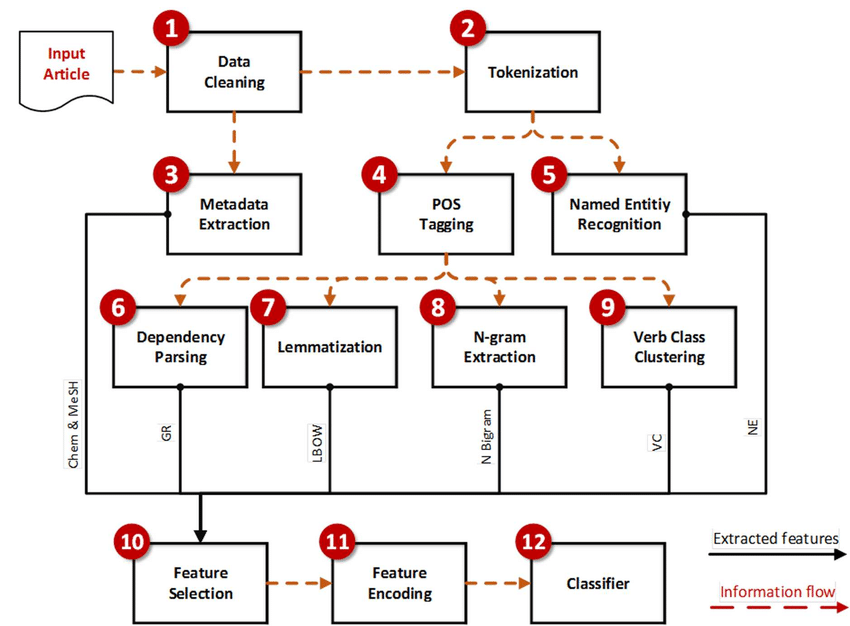
\includegraphics[width=\textwidth]{media/The-NLP-pipeline-for-automatic-classification-of-document-abstracts-Chem-Chemical.png}
    \caption{Caption}
    \label{fig:my_label}
\end{figure}

The table \ref{table:1} is an example of referenced \LaTeX elements.

\begin{table}[h!]
\centering
\begin{tabular}{||c c c c||} 
 \hline
 Col1 & Col2 & Col2 & Col3 \\ [0.5ex] 
 \hline\hline
 1 & 6 & 87837 & 787 \\ 
 2 & 7 & 78 & 5415 \\
 3 & 545 & 778 & 7507 \\
 4 & 545 & 18744 & 7560 \\
 5 & 88 & 788 & 6344 \\ [1ex] 
 \hline
\end{tabular}
\caption{Table to test captions and labels}
\label{table:1}
\end{table}
